\section{Neural Networks}

\subsection{Backpropagation}
"Backpropagation is the algorithm for determining how a single training example would like to nudge the weights and biases (Gradient-based update), not just in terms of whether they should increase or decrease, but also in terms of the relative proportions that would cause the most rapid decrease in the cost function (Gradient direction). A true gradient descent step would involve computing these adjustments for all tens of thousands of training examples and averaging the resulting gradients. However, this is computationally expensive, so instead, the training data is randomly subdivided into mini-batches, and each gradient descent step is computed with respect to one mini-batch at a time. By repeatedly going through all of the mini-batches (Epoch) and updating the weights accordingly, the network gradually converges toward a local minimum of the cost function. In doing so, the network ends up performing very well on the training examples."


\textbf{Useful Terms:}
\begin{itemize}
    \item \textbf{Mini-batch:} A small subset of the training data used to compute the gradient for a single update step.
    \item \textbf{Batch Size:} The number of training examples in a mini-batch (hyperparameter).
    \item \textbf{Epoch:} One complete pass through the entire training dataset (via all mini-batches).
    \item \textbf{Dropout (rate):} A regularization technique where a fraction of neurons are randomly set to zero during a batch training to prevent overfitting. The rate is an hyperparameter (usually 50\%).
\end{itemize}

\begin{center}
    \textbf{Training Pipeline:}

    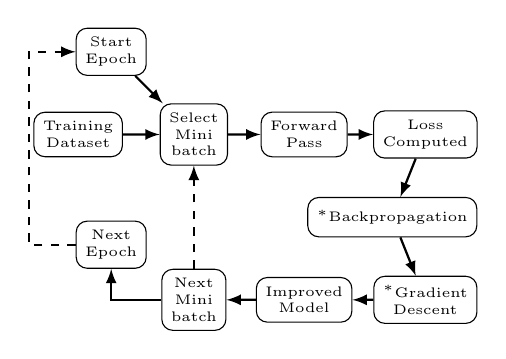
\begin{tikzpicture}[scale=0.7,
        every node/.style={draw, rounded corners, align=center, font=\tiny,
                minimum width=0.8cm, minimum height=0.5cm},
        arrow/.style={-{latex}, thick},
        dloop/.style={-{latex}, thick, dashed}
        ]

        % ---------------- Main pipeline ----------------
        \node (dataset)  at (-2.6,  1.5) {Training\\Dataset};
        \node (batch)    at ( -0.5,1.5) {Select\\Mini\\batch};
        \node (forward)  at ( 1.5,1.5) {Forward\\Pass};
        \node (loss)     at ( 3.7,1.5) {Loss\\Computed};
        \node (backprop) at ( 3.1,0)   {$^*$Backpropagation};
        \node (update)   at ( 3.7,-1.5){$^*$Gradient\\Descent};
        \node (improved) at ( 1.5,-1.5){Improved\\Model};

        % ---------------- Loop-control nodes -----------
        \node (nextbatch) at (-0.5,-1.5) {Next\\Mini\\batch};
        \node (epoch)     at (-2, 3)    {Start\\Epoch};
        \node (nextepoch) at (-2,-0.5)  {Next\\Epoch};

        % ---------------- Straight arrows --------------
        \draw[arrow] (dataset)  -- (batch);
        \draw[arrow] (batch)    -- (forward);
        \draw[arrow] (forward)  -- (loss);
        \draw[arrow] (loss)     -- (backprop);
        \draw[arrow] (backprop) -- (update);
        \draw[arrow] (update)   -- (improved);
        \draw[arrow] (improved) -- (nextbatch);

        % ---------------- Mini-batch loop (dashed) -----
        \draw[dloop] (nextbatch.north) -- (batch.south);

        % ---------------- Epoch loop (dashed) ----------
        \draw[arrow] (nextbatch.west) -- ++(-0.50,0) -| (nextepoch.south);      % end of last mini-batch
        \draw[dloop] (nextepoch.west) -- ++(-0.85,0) |- (epoch.west);
        \draw[arrow] (epoch) -- (batch);              % new epoch begins

    \end{tikzpicture}

    \textit{$^*$Backpropagation computes gradients; a gradient-based optimiser applies them over many mini-batches and epochs.}

\end{center}


\subsection{FNNs (Feedforward Neural Networks)}

\subsection{CNNs (Convolutional Neural Networks)}

\subsection{RNNs (Recurrent Neural Networks)}

RNNs process sequential data, using previous steps to inform current predictions. Useful for text, audio, etc. and supports one/many-to-one/many sequence I/O patterns (e.g image $\to$ description is one-to-many).

$h_t = \tanh(U h_{t-1} + V x_t)$

\subsubsection{Basic RNN}
\textbf{Diagrams notation:}
\begin{center}
    % https://colah.github.io/posts/2015-08-Understanding-LSTMs
    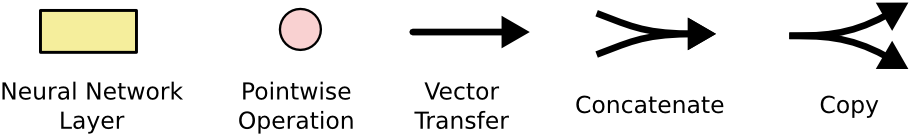
\includegraphics[width=0.98\columnwidth]{images/rnn_notations.png}
\end{center}

\textbf{RNN Cell:}
\begin{center}
    % https://colah.github.io/posts/2015-08-Understanding-LSTMs
    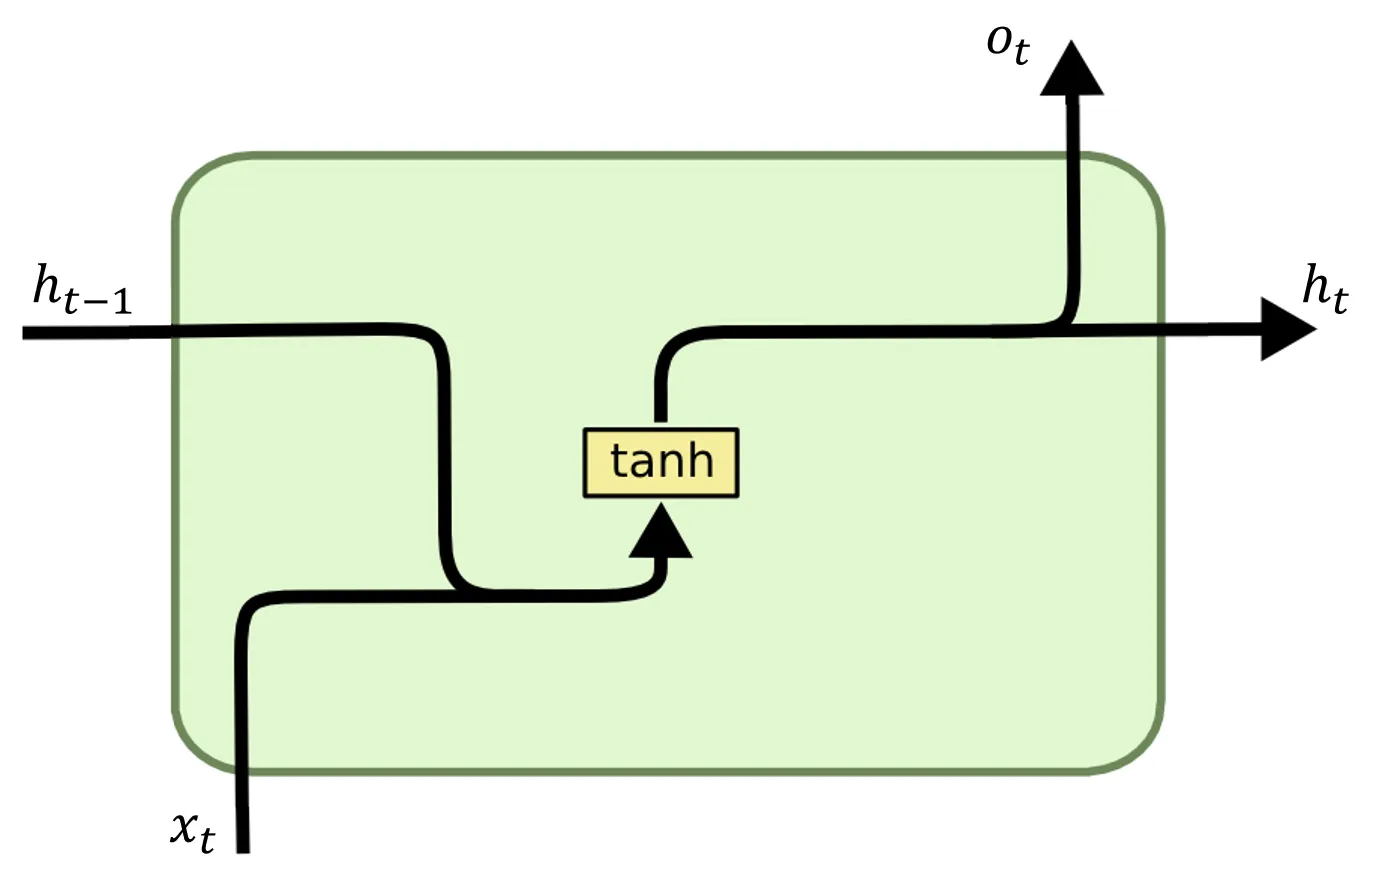
\includegraphics[width=0.98\columnwidth]{images/rnn_cell.png}
\end{center}

\subsubsection{Long Short-Term Memory (LSTM)}

LSTMs are a type of RNN designed to remember information for long periods, addressing the vanishing gradient problem. They achieve this through a cell state ($C_t$) and three gates: input ($i_t$), forget ($f_t$), and output ($o_t$).

\begin{center}
    % https://colah.github.io/posts/2015-08-Understanding-LSTMs
    % LSTM Cell Diagram with included title
    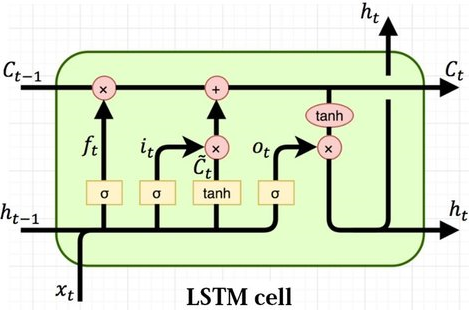
\includegraphics[width=0.98\columnwidth]{images/lstm_cell_trim.png}
\end{center}

\text{Where:}
\begin{itemize}
    \item $i_t = \sigma(x_t U^i + h_{t-1} W^i) \quad$ Input gate, controls how much of the input to let through.
    \item $f_t = \sigma(x_t U^f + h_{t-1} W^f) \quad$ Forget gate, controls how much of the previous cell state to keep.
    \item $o_t = \sigma(x_t U^o + h_{t-1} W^o) \quad$ Output gate, controls how much of the cell state to output.
    \item $\tilde{c}_t = \tanh(x_t U^g + h_{t-1} W^g) \quad$ Candidate cell state, potential new information to add to the cell state.
    \item $c_t = \sigma(f_t * C_{t-1} + i_t * \tilde{C}_t) \quad$ Cell state, memory of the LSTM.
    \item $h_t = \tanh(C_t) * o_t \quad$ Hidden state, output of the LSTM at time $t$.
\end{itemize}

\textbf{LSTM Chain:}
\begin{center}
    % https://colah.github.io/posts/2015-08-Understanding-LSTMs
    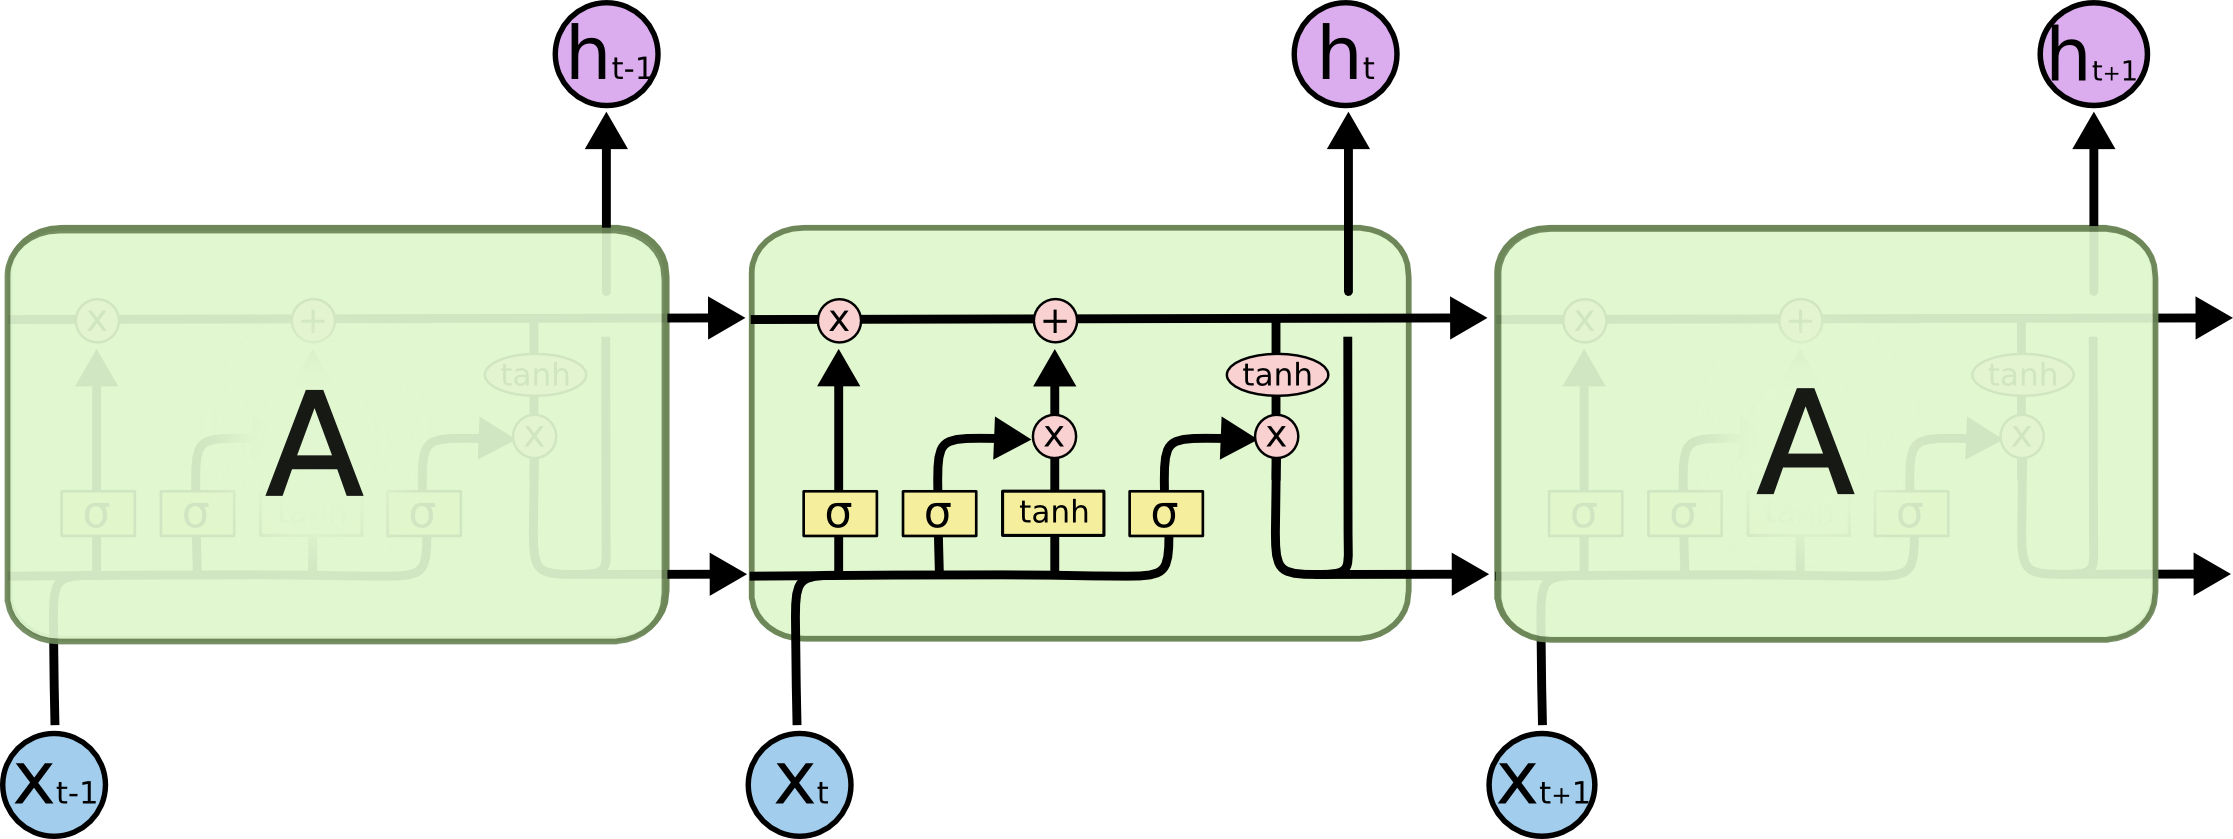
\includegraphics[width=0.98\columnwidth]{images/lstm-chain.png}
\end{center}

\subsubsection{RNNs vs. CNNs}
\begin{center}
    \resizebox{\columnwidth}{!}{
    \begin{tabular}{lcc}
        \hline
        \textbf{Property}                    & \textbf{RNN}     & \textbf{CNN} \\
        \hline
        Long-range mechanism                 & Gating/Attention & Pooling      \\
        Sequential                           & $+$              & $-$          \\
        Parallelizable                       & $-$              & $+$          \\
        Compute time for $n$ tokens          & $O(n\cdot L)$    & $O(L)$       \\
        Layers required for the $n$-th token & $1$              & $\log n$     \\
        \hline
    \end{tabular}
    }
\end{center}